\section{实验}
\label{sec:experiments}
%% =====================================================================

\subsection{协议}
\label{sec:protocol}

\textbf{路网、路由与算例。}
下层路网、时间窗路由与独立校验器固定。扩样矩阵使用\textbf{五个算例}：
小例 \texttt{example\_3x3x2}、拥堵例 \texttt{congested\_8x4x4}，
以及三个 \texttt{S8x4x4} 布局 \texttt{high}、\texttt{funnel} 与 \texttt{mid}。
后三者同规模、同柔性，只差走廊拓扑，因此它们之间预约影响集规模的差异可归因于拓扑而非问题尺寸。
五者分两种来源：前两个是手写布局（小例供逐步核对，拥堵例为哑铃拓扑）；后三个由本文的算例
生成器产生，其参数（工件数 \(\times\) 机器数 \(\times\) AGV 数、拥堵档、异构度 \(h\)、柔性度 \(f\)）
与\textbf{生成随机种子}一并编码在算例文件名中，三者的生成随机种子同为 \(42\)。
\textbf{生成随机种子与下文的运行随机种子相互独立}：前者只决定算例本身，后者决定扰动注入
与搜索过程；两者取值中均含 \(42\)，但并无共用。
\textbf{运行随机种子取十个}，即 \(42\)、\(7\)、\(2024\)、\(99\)、\(123\)、\(13\)、\(1\)、
\(777\)、\(31415\) 与 \(8\)，共 \(\NInst\times\NSeeds=\NPairs\) 个算例--随机种子对，下文每一对称为一「格」。
全文所有逐格比较、胜负计数与配对检验都按（算例，随机种子）这一对键对齐：
同一键下各方法读取同一份初始解、同一段阻断与同一决策时刻。
初始排程由第~\ref{sec:reservation}~节的时间窗路由按加工顺序重放得到，
并通过独立无冲突校验；同一算例--随机种子对下各对照方法共享该初始解。
对 \(\mathcal{S}^0\) 只要求其在扰动前可行。

\textbf{实现与运行环境。}
全部实验为纯 Python 标准库实现，不依赖第三方数值库；下层路网、时间窗路由与独立校验器
复用与静态一体化工作同一份实现。单机单线程运行，不使用并行：Intel Xeon W-1270
（\(8\) 核 \(16\) 线程）、\(64\)\,GB 内存、Windows 10，解释器为 CPython \(3.7.6\)（\(64\) 位）。
因不引入第三方数值库，复现不需要锁定依赖版本；\(3.7\) 是本文实测的解释器，
更高版本未逐一复跑。所有计时结果都在上述单机单线程条件下取得，
更换硬件会使其整体平移，故本文的耗时结论均以\emph{比值}或\emph{量级}形式给出，不依赖绝对毫秒数。

\textbf{代码与数据可用性。}
复现所需材料分三部分：上层有界修复与实验驱动、下层路网与时间窗路由、
算例与扰动输入及全部逐格结果(CSV)。三者连同生成各表各图的脚本一并提交，
审稿期间以\textbf{匿名仓库}形式提供（见投稿系统所附链接，仓库内不含作者身份信息）；
论文接受后转为公开仓库并在永久存档服务上登记 DOI，本节届时补填该 DOI。
每张表与每幅图在仓库中都能追到生成它的脚本与对应的 CSV，
表~\ref{tab:instscale} 所列算例亦随仓库分发。

\textbf{第二批：布局出处外部化。}
上面五个算例的布局都是本文设计的，其中三张同规模布局还同属哑铃一族（彼此只差装卸站
出口与中段的并行通道数，即只差容量、不差几何）。为使布局不由本文决定，另外运行一批
\NPubInst\ 个算例：路网的网格尺寸、装卸站与机器落位、缺失的边这三项逐项转录自
Lyu 等~\cite{lyu2019approach} 附录 A 的布局图，转录结果由脚本与 van Os 配套工具集
所给的机读编码逐字段对账。机器台数因此由布局决定而非由本文选定，为 \(4\) 至 \(8\) 台。
随机种子仍取同样十个，合计 \NPubPairs\ 个算例--随机种子对。两批算例\emph{逐参数同口径}：工件数、
AGV 数、每工件工序数、\(h\)、\(f\) 以及运输/加工时长比的标定目标一律相同，因此两批之差
可唯一归因于布局出处。

该附录共给出六张布局（\(3\) 至 \(8\) 机）。\(3\) 机布局未采用：固定 \(f=0.6\) 在 \(|M|=3\) 时
平均候选机数为 \(1.8<2\)，与「每道工序至少两台候选机」不相容，而为单张布局放宽 \(f\)
会引入额外变量。

其余五张\textbf{只落在 \NPubNets\ 张不同路网上}：\(4\) 机与 \(5\) 机两张共用
同一张 \(4\times 4\) 网格（去掉同一条边），\(6\)、\(7\)、\(8\) 机三张共用同一张
\(5\times 5\) 网格（去掉同两条边）；五者彼此的差别在于机器台数与\emph{落位}，
而非路网几何（原始发布数据即如此组织）。因此第~\ref{sec:e4}~节分析这批
数据时，\textbf{路网几何这一维的独立样本数是 \NPubNets\ 而非 \NPubInst}，机器落位这一维则
有 \NPubInst\ 个；下文的论断均按此划分给出。

该批算例有三处与原始数据不同。\textbf{其一，逐段行驶时间不是原始数据。} Lyu 只为单个示例
算例发表过逐段时长，且其取值并不均匀；附录 A 那批布局的逐段时长从未发表。故这里按
「所有边等权」补齐——它与 van Os 模型里「单步时长为常量」的假设在结构上一致，只是时间单位的
标度不同。因此本批结果不与 Lyu 或 van Os 的参照值比较，仅作为一批非本文设计的拓扑使用。\textbf{其二，装卸站做了合并。} 原布局有分离
的装货站与卸货站，本文只有一个装卸站，故取车辆起始处的装货站作为装卸站，卸货站视为普通
网格节点。\textbf{其三，未采用其工件数据。} 在已实测的公开算例族中，平均运输时长只占平均
加工时长的百分之几，运输几乎不构成争用；若同时采用其工件数据，走廊争用及以其为对象的
全部现象都将无法观察。因此外部化的只有路网。
同一工具集另附的一族布局（其目录标注为 Liu 2023）未纳入本批：这些布局允许对角
移动，而本文的走廊为四邻接；支持对角移动需要修改下层路由，而非算例。

\textbf{扰动。}
除非另注，\(t_{\mathrm{now}}=0.35\,C_{\max}(\mathcal{S}^0)\)。
E1--E3 与 E5 在繁忙走廊上施加单窗阻断；E6 在同一 \(t_{\mathrm{now}}\) 上另加三类扰动；
E4 阻断 LU 割中的走廊（第~\ref{sec:e4}~节）；
扰动规模扫描将未来工序按最早未来预约排序，取前比例 \(\varphi\) 的预约时窗作为微阻断（不合并）。

\textbf{对照方法。}
R1：按工序依赖图上的影响域划界 + 第 1 级改路，全文取 \(\theta=2\)
（该值只影响 A 类扰动下 \(|U_{R1}|\) 的大小；由命题~\ref{prop:miss},B 类上
任何有限 \(\theta\) 都给出空集）；其划界规则取自第~\ref{sec:rw_aor}~节所述的工序级
局部重调度做法，由本文重新实现。逐条对应关系是：「受影响工序集取直接受扰工序，
再沿工件内工序先后关系向后扩张」这一条划界规则对应
AOR~\cite{abumaizar1997rescheduling,subramaniam2003maor}；
而\emph{以跳数 \(\theta\) 截断扩张}、以及\emph{把工序集映射为须释放的走廊预约}
两项由本文写定——原文的设定里没有预约表，这一映射在原文中无对应物；
改路与重放部件则与 R2 共用同一份实现，以保证两者只差划界对象。
因此 R1 是将该划界规则移植到本文预约设定下的对照，其结果反映该规则在此设定下的表现，
而非原方法在其自身设定下的表现；
R2/\STRC：按预约影响集划界 + 第 1 级改路（规模扫描打开失败后扩大范围；E3/E5 关闭这一步）；
R0+：以原排程为起点、在限定时间内重新搜索的全局重调度——遗传算法，种群 \(40\)，
原排程对应的染色体置入初始种群，解码采用与 RD 相同的固定前缀解码（\(t_{\mathrm{now}}\)
之前的占用不可改写）；\emph{不设代数上限与早停阈值}，终止条件只有挂钟预算一项，
预算取值见第~\ref{sec:e5}~节；
RS：全局右移，不按影响集划界且不改路（第~\ref{sec:cheap}~节）；
RD：原染色体重解码，即本实现中耗时最短的全局重算（同节）；
RA：不按影响集限制范围但保留改路，即把 \(t_{\mathrm{now}}\) 之后尚未结束的占用全部纳入改写，其余与 R2 逐项相同，
用于单独检验预约影响集的作用（同节）。
这五条对照按「是否划界 \(\times\) 重算范围」组织：R1 与 R2 只差划界\emph{对象},
RA 与 R2 只差\emph{是否}划界（改路程序完全相同），RS 既不划界又放弃改路而整体后推，
RD 与 R0+ 则重算全局而不按影响集划界，只差搜索多少代。

\textbf{预算口径。}
各方法不在同一预算档上比较：R1、R2、RS、RD、RA 均为一次确定性修复，
运行结束即终止，耗时由算例规模与影响集大小决定而非由预算设定；只有 R0+ 按挂钟预算终止。
因此涉及 R0+ 的结果均为给定预算下的结果；第~\ref{sec:cheap}~节的四法对照才是同一预算档内
（均运行一次即终止）的比较。挂钟耗时按批次报告，不跨批次比较。

\textbf{失败后扩大范围的开关。}
E3 中关闭失败后扩大范围。若开启，R1 可能在扩大到全部尚未结束的占用后恢复可行，
测得的将是扩大规则的回退能力，而不是划界对象的差别。扩大范围本身有效（规模扫描中它使全部格
恢复可行），但它与被测变量无关，故在边界消融中关闭。
其端点即第~\ref{sec:cheap}~节的 RA，该节将其作为独立对照逐格测量代价。

\textbf{两批算例的分工。}
两批并非同一组证据的两次采样，它们回答的问题不同。
主批次回答\emph{现象是否存在、机制能否被单独识别}:B 类扰动下按工序依赖图划界得到空范围而原排程不可行
（第~\ref{sec:e1}~节）、预约影响集对该范围的包含与集外字段的不变性（第~\ref{sec:e2}~节）、
同一套改路程序下只替换划界对象的对照（第~\ref{sec:e3}~节）。这三项都要求完全控制算例参数，
尤其是决定走廊争用是否成立的运输/加工时长比，而公开算例族无法提供这种控制
（第~\ref{sec:limitations}~节局限第 4 条）。第二批回答另一个问题：\emph{这些现象
是否只在本文自选的布局上成立}。它主要用于复现（第~\ref{sec:pubrepro}~节），
不产生新的性能对比结论。

两批合并分析的只有两处。其一是 E4：主批次的三张同规模布局同属一族、几何差异很小，
「指标过粗」与「算例几何差异不足」两种解释无法区分；而外部布局若没有逐参数同口径的
自建对照，也无从判断其影响集占比的变动幅度是否足够大。第二批据此收窄了结构可预测性的结论。
其二是 E5：两批的 E5 协议与参数逐项相同，合并只为增加格数，不改变结论方向。
其余各节的结论由主批次单独给出，第二批只增强其外部效度。

\textbf{统计口径。}
全文有两处推断性检验，均在第~\ref{sec:cheap}~节：R2 与 RA 在改动比例上的差（主检验），
以及 R2 与 RD 在完工时间上的差。二者均采用 Wilcoxon 符号秩检验，双侧，按上述（算例，随机种子）键配对。
按 Holm 法对这两次检验校正后，各自的显著性判断不变；其余各处的逐格胜负、均值与中位数
均为\emph{描述性}统计，不作显著性断言。
该检验配套的效应量报为 Hodges--Lehmann 估计 \(0.037\),\(95\%\) 自助置信区间
\([0.018,\,0.074]\)（百分位法，\(10^4\) 次重采样，固定随机种子）；配对差的均值为
\(\RAStabMean\)，区间 \([0.039,\,0.093]\)。离散度按四分位距报告：改动比例在 R2 上为
\(0.073\)、在 RA 上为 \(0.062\)。
% selfcheck:allow-num 0.073 为 R2 改动比例的四分位距,与 \RAStabMeanNet(剔除恒等格后的平均降幅)同值不同源
由于 \(50\) 格中有 \(18\) 格两法恰好持平，配对差\emph{中位数}的置信区间下端为 \(0\)；
这表明持平格约占胜负计数的三分之一。
其余各批次的表格只给均值、中位与计数，不含区间。

\subsection{E1：工序依赖图给出空范围}
\label{sec:e1}

本节只考察 B 类扰动下两种划界各给出什么范围，不比较修复质量。
表~\ref{tab:e1} 与图~\ref{fig:e1e3}（左）按第~\ref{sec:protocol}~节的走廊阻断协议汇总命题~\ref{prop:miss} 的扩样结果：
在 \(\PassMiss\) 格上，\(T_{\mathrm{impact}}=0\)、起点占用与预约影响集非空、阻断后原排程不可行。

表~\ref{tab:e1} 把三个条件合并计入「三条件通过」一列（逐格结果见 \texttt{e1\_miss.csv} 的
\texttt{n\_T\_impact} 与 \texttt{feasible\_after\_block} 两列）。
其中 \(T_{\mathrm{impact}}=0\) 由定义~\ref{def:task_impact} 对 B 类的约定直接得到；
实质性的结果是后一列恒为假，即原排程\emph{确实}已不可行，两者合起来构成反例。

\begin{table}[t]
\centering
\caption{E1 走廊阻断下工序依赖图给出空范围（每算例 \(\NSeeds\) 个随机种子，共 \(\NPairs\) 对）。
\(|R|\) 为全表占用数，\(\mathrm{Cl}/|R|\) 为预约影响集占全表的比例。均值取多个随机种子的平均。
离散度按四分位距(IQR)报告：逐算例 \(\mathrm{Cl}/|R|\) 的 IQR 在
\EoneFracIqrLo--\EoneFracIqrHi 之间，\(\NPairs\) 对合池的中位为 \EoneFracMed、
极差 \EoneFracMin--\EoneFracMax；可见该比例的算例间差异与随机种子间差异同量级，
不宜只读均值。
「三条件通过」为命题~\ref{prop:miss} 三条件同时成立的格数（\(T_{\mathrm{impact}}=0\)、
起点占用非空、阻断后原排程不可行）。后三行同规模同柔性，只差走廊拓扑。}
\label{tab:e1}
\small
\begin{tabular}{@{}lcccccc@{}}
\toprule
算例 & 随机种子 & 三条件通过 & 均 \(|R|\) & 均 \(|\mathrm{Src}|\)
 & 均 \(|\mathrm{Cl}|\) & \(\mathrm{Cl}/|R|\) \\
\midrule
\texttt{example\_3x3x2}   & 10 & \(10/10\) & \(28.6\)  & \(5.6\)  & \(16.9\) & \(0.59\) \\
\texttt{congested\_8x4x4} & 10 & \(10/10\) & \(85.0\)  & \(15.0\) & \(48.4\) & \(0.57\) \\
\texttt{S8x4x4} (high)    & 10 & \(10/10\) & \(150.5\) & \(15.5\) & \(88.3\) & \(0.59\) \\
\texttt{S8x4x4} (funnel)  & 10 & \(10/10\) & \(149.1\) & \(15.5\) & \(85.4\) & \(0.57\) \\
\texttt{S8x4x4} (mid)     & 10 & \(10/10\) & \(147.6\) & \(15.0\) & \(82.8\) & \(0.56\) \\
\midrule
合计 & \(\NPairs\) & \(\PassMiss\) & --- & --- & --- & --- \\
\bottomrule
\end{tabular}
\end{table}

\(|\mathrm{Cl}|\) 的绝对值随算例变大(\(16.9\)、\(48.4\)、\(82.8\)--\(88.3\))，这是占用总数变多的直接结果；
而 \(\mathrm{Cl}/|R|\) 在五个算例上都落在 \EoneCloLo--\EoneCloHi,\emph{未能}区分三个 \(\texttt{S8x4x4}\) 布局。
这与第~\ref{sec:e4}~节的结论一致：实验没有给出能可靠预测影响集规模的结构指标。
就贡献而言，本节支撑 C1:B 类扰动下按工序依赖图划界得到空范围，而原排程已不可行。

\subsection{E2：包含性}
\label{sec:e2}

结构闭合性(E2a)在 \(\PassClosed\) 格上成立（泄漏 \(=0\)），与命题~\ref{prop:struct} 一致。
第 1 级修复（不扩大范围）在 \(\NPairs/\NPairs\) 格上可行。
集外占用的走廊、时段与车辆逐条不变（E2b，即命题~\ref{prop:outside} 的观测形式）同样在 \(\PassInvar\) 格上
成立（表~\ref{tab:e2}）。

\begin{table}[t]
\centering
\caption{E2 包含性（\(\NSeeds\) 个随机种子/算例；第 1 级可行一列不扩大范围）。
E2a 为结构闭合（泄漏 \(=0\)），
E2b 为集外占用的走廊、时段与车辆\emph{逐条}不变。}
\label{tab:e2}
\small
\begin{tabular}{@{}lccc@{}}
\toprule
算例 & E2a 闭合 & 第 1 级可行 & E2b 集外逐条不变 \\
\midrule
\texttt{example\_3x3x2}   & \(10/10\) & \(10/10\) & \(10/10\) \\
\texttt{congested\_8x4x4} & \(10/10\) & \(10/10\) & \(10/10\) \\
\texttt{S8x4x4} (high)    & \(10/10\) & \(10/10\) & \(10/10\) \\
\texttt{S8x4x4} (funnel)  & \(10/10\) & \(10/10\) & \(10/10\) \\
\texttt{S8x4x4} (mid)     & \(10/10\) & \(10/10\) & \(10/10\) \\
\midrule
合计 & \(\PassClosed\) & \(\NPairs/\NPairs\) & \(\PassInvar\) \\
\bottomrule
\end{tabular}
\end{table}

E2a 与 E2b 含义不同。E2a 是\emph{图上的}性质，由命题~\ref{prop:struct} 保证，
用于检验实现与定义是否一致；E2b 是\emph{修复之后的}性质，检验命题~\ref{prop:outside} 的四条前提
在本文协议下是否成立。其中前提 (ii) 要求集外占用逐条预提交成功；若某条集外占用与禁行窗重叠，
预提交即失败，说明起点占用集不完备（注~\ref{rem:precommit}）。
就贡献而言，E1、E2 与第~\ref{sec:e3}~节的边界消融支撑 C1 与 C2 的\emph{对象层}：预约影响集
由边集唯一确定、对外封闭，且在同一套改路程序下均恢复了可行；划界的净收益由
第~\ref{sec:cheap}~节的 RA 对照给出。

\begin{remark}[实现缺陷被误读为边集缺陷的一例]
\label{rem:e2b_history}
若按\emph{工序}而非\emph{占用}判定是否改路，E2b 仅在 \(24/\NPairs\) 格上通过，
容易被误读为「依赖边集未能覆盖若干弱耦合」。其实际原因是粒度错配：允许改写的是\emph{占用}集合，
而按工序判定时，同一工序的空载段与满载段只要有一段落在影响集内，整道运输就被重新规划。
当只有满载段进入影响集时，同工序的空载段也被改写，而它的任务标签不在允许改写的集合内，
因而被记为集外漂移。\(26\) 个未通过格上的 \(84\) 条漂移占用全部属于这种同工序空载段，
其中 \(71\) 条(\(85\%\))在 \(t_{\mathrm{now}}\) 之前已执行完毕，改写它们同时违反假设 A2。
改为按\emph{段}判定（已执行完或未纳入改写的空载段沿用原计划，
只对落在允许改写集合内的段改路）之后，漂移归零。
可见此时测得的不是边集对物理耦合的覆盖程度，而是命题~\ref{prop:outside} 前提 (iii)
「仅对 \(U\) 内运输调用路由器」在实现上未被满足。
这一误判的一般形式是：把实现与定义之间的粒度错配，误读为模型刻画能力的不足。

\textbf{E2b 无法检出的同类错配。} 按段判定时，一个\emph{跨越}
\(t_{\mathrm{now}}\) 的运输段仍整段重新规划：只要它有一个路段的结束时刻晚于
\(t_{\mathrm{now}}\)，整段的任务标签就进入允许改写的集合，于是它在 \(t_{\mathrm{now}}\)
之前\emph{已通过}的路段也被重排，相当于让车辆回到该段起点重新行驶，违反假设 A2。
E2b 无法检出这一情形，因为这些路段的任务标签位于影响集\emph{内}，不在集外字段的比对范围中。
这一情形由一项独立的已完成占用审计（逐条比对 \(t^e\le t_{\mathrm{now}}\)
的占用）检出：\(\NPairs\) 格中有 \(36\) 格存在此类改写，合计 \(86\) 条。
将粒度细化到\emph{路段}（已通过的路段原样保留，改路只从车辆在
\(t_{\mathrm{now}}\) 时实际所在的节点开始）之后，该审计在全部 \(\NPairs\) 格上归零，
各项通过率不变，\(C_{\max}\) 在 \(6\) 格上改善、无一格变差。
本文各表报告的均为按路段粒度实现的结果；本注中的数字（\(24/\NPairs\)、\(26\) 格 \(84\) 条、\(36\) 格 \(86\) 条）
均来自较粗粒度的实现。
\end{remark}

\subsection{E3：边界消融}
\label{sec:e3}

表~\ref{tab:e3} 与图~\ref{fig:e1e3}（右）固定第 1 级改路并\emph{关闭}失败后扩大范围。
B 类扰动下，R1 在 \(\NPairs/\NPairs\) 格上的允许改写集合为空且不可行，R2 全部可行。

两臂使用同一套改路程序、同一份初始解、同一个 \(t_{\mathrm{now}}\)、同一批随机种子与同一段阻断窗，
\textbf{唯一的差别是允许改写哪些占用}。R1 的允许改写集合为空，第 1 级改路对空集是恒等操作，
原排程保持不变，仍占用被阻断的走廊；因此 R1 的失败来自它判定无需重调度，而非修复质量。
第 1 级改路逐格的耗时中位数为 \(\MsRepairMed\)\,ms、最大 \(\MsRepairMax\)\,ms；表~\ref{tab:e3} 末列
是各算例内 \(\NSeeds\) 个随机种子的均值，两者口径不同，不可直接比较。
就贡献而言，本节把缺口的成因归于划界对象(C2、C3)：同一套改路程序只替换划界对象，恢复可行率即从
\(\FeasRone\) 变为 \(\FeasRtwo\)。

上述反差是否依赖边权标定，另作检验。本文的走廊边权取等权，故按三档非均匀边权
（\texttt{lognormal}、\texttt{lu\_far}、\texttt{split}；数据见 \texttt{weight\_sweep.csv}）
在同一批 \(\NPairs\) 对上重新运行 E1 与 E3：三条件通过与工序依赖图范围为空的结果逐档不变，
R1 仍全格不可行，R2 第 1 级的可行格数依次为 \WeightLogRtwo、\WeightLuRtwo、\WeightSplitRtwo，
唯一不可行的一格出现在 \texttt{split} 档（\texttt{S8x4x4\_high}，随机种子 \(1\)）。
故该反差不依赖等权这一标定。

\begin{table}[t]
\centering
\caption{E3 边界消融（不扩大范围；\(\NInst\) 算例 \(\times\) \(\NSeeds\) 个随机种子）。
miss\_B 指该格上 R1 的允许改写集合为空而 R2 非空。
末列为各算例内 \(\NSeeds\) 个随机种子的均值，与正文逐格中位数口径不同。}
\label{tab:e3}
\small
\begin{tabular}{@{}lccccc@{}}
\toprule
算例 & miss\_B & R1 可行 & R2 可行 & 均 \(|U_{R2}|\) & R2 耗时/ms \\
\midrule
\texttt{example\_3x3x2}   & \(10/10\) & \(0/10\) & \(10/10\) & \(16.9\) & \(0.66\) \\
\texttt{congested\_8x4x4} & \(10/10\) & \(0/10\) & \(10/10\) & \(48.4\) & \(2.84\) \\
\texttt{S8x4x4} (high)    & \(10/10\) & \(0/10\) & \(10/10\) & \(88.3\) & \(3.40\) \\
\texttt{S8x4x4} (funnel)  & \(10/10\) & \(0/10\) & \(10/10\) & \(85.4\) & \(5.09\) \\
\texttt{S8x4x4} (mid)     & \(10/10\) & \(0/10\) & \(10/10\) & \(82.8\) & \(3.96\) \\
\midrule
合计 & \(\NPairs/\NPairs\) & \(\FeasRone\) & \(\FeasRtwo\) & --- & --- \\
\bottomrule
\end{tabular}
\end{table}

\begin{figure}[t]
\centering
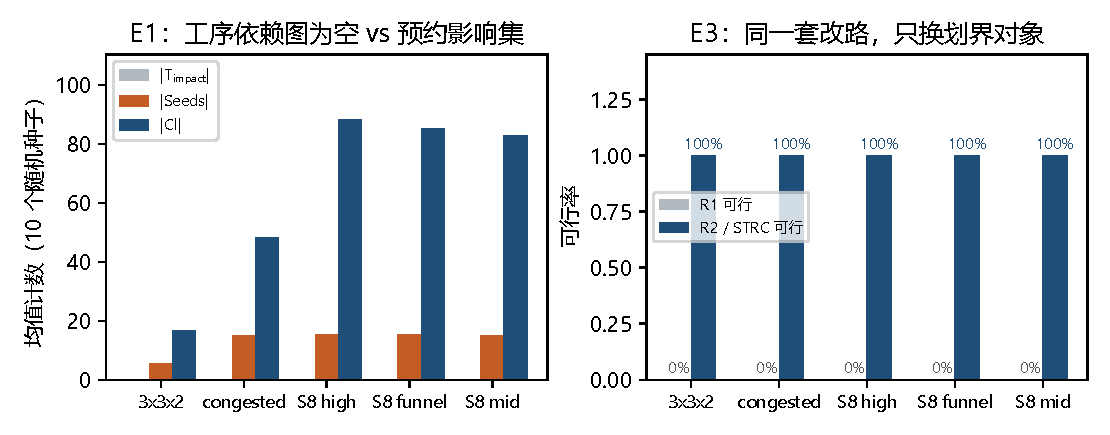
\includegraphics[width=\linewidth]{figures/fig_strc_e1e3_CN}
\caption{E1/E3 扩样可视化（\(\NInst\) 算例 \(\times\) \(\NSeeds\) 个随机种子均值）。
左：工序依赖图上的影响域为空，而起点占用与预约影响集非空；柱高为每算例 \(\NSeeds\) 格
的均值，离散度按四分位距见表~\ref{tab:e1}（\(|\mathrm{Cl}|\) 的 IQR 逐算例在 \(2\)--\(8\)
之间，影响域一组恒为零故无离散度）。
右：同一套改路、只换划界对象时 R1 可行率为 \(0\)、R2 为 \(100\%\)；该幅为逐格计数
（各 \(\NPairs\) 格），故不给出离散度。}
\Description{并排两幅条形图。左幅按五个算例给出工序依赖图影响域、起点占用数与预约影响集规模
三组柱子，影响域一组恒为零，另两组随算例规模上升。右幅给出两种划界的恢复
可行率，按工序依赖图划界一侧为零，按预约影响集划界一侧为百分之百。}
\label{fig:e1e3}
\end{figure}

\subsection{案例甘特图}
\label{sec:case}

\begin{sloppypar}
E1--E3 给出的是跨随机种子的计数与可行率。为在工序时间轴上展示「工序依赖图无法刻画、按预约影响集可以修复」的情形，
图~\ref{fig:case} 取 \texttt{example\_3x3x2}、随机种子 \(42\) 的一例走廊阻断，
协议同 E2/E3：决策时刻取 \(0.35\,C_{\max}\)，繁忙走廊单窗阻断，第 1 级改路、不扩大范围。
\end{sloppypar}

该例上 \(T_{\mathrm{impact}}=\varnothing\)，而 \(|\mathrm{Src}|=6\)、\(|\mathrm{Cl}|=18\)。
图~\ref{fig:case}(a) 为扰动前原排程的机器甘特图：蓝色工序的运输占用落入影响集（将被改路），
灰色工序在影响集外（预提交、保持原计划）；红色虚线为 \(t_{\mathrm{now}}\)，浅红带为阻断时窗。
图~\ref{fig:case}(b) 为修复后：影响集内工序时间轴重排，排程在阻断下恢复可行，
\(C_{\max}:57\to 86\)，耗时亚毫秒级。
本图只说明统计结论对应何种局部改动形态，不用于比较完工时间；
完工时间与全局重调度的权衡见 E5 与扰动规模扫描。

\begin{figure}[t]
\centering
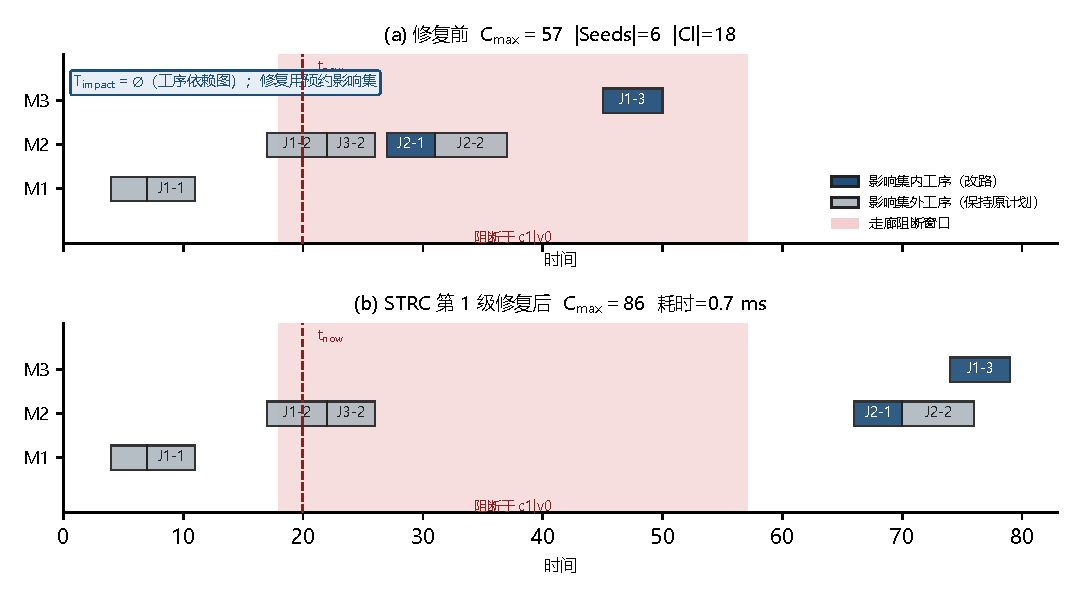
\includegraphics[width=\linewidth]{figures/fig_strc_case_CN}
\caption{案例甘特图（\texttt{example\_3x3x2}，随机种子 \(42\)）。
(a)~阻断前原排程，按是否属于 \(\mathrm{Cl}\) 着色；
(b)~第 1 级修复后。工序依赖图上的影响域为空；蓝色工序对应影响集内运输被改路。
本图仅示意局部改动的形态。}
\Description{上下两幅机器甘特图。(a) 阻断前的原排程，条块按其运输占用是否落在
预约影响集内着蓝灰两色，一条竖直红虚线标出决策时刻，一条浅红竖带标出阻断时窗。
(b) 修复后的排程，蓝色条块的时间轴被重排，灰色条块位置不变，完工时间由 57 增至 86。}
\label{fig:case}
\end{figure}

